\chapter{What Is Economics? (Text Ch. 1)}

\section{Definition of economics}

Every economic question arises because we want more than we can get. Our wants are
effectively unlimited, but the time, resources and technology available to satisfy them
are limited.

\begin{definition}[Scarcity]
\emph{Scarcity} is our inability to satisfy all of our wants. Because of scarcity we must
make \emph{choices}: getting more of one thing means getting less of something else.
\end{definition}

Scarcity is not the same as poverty. A billionaire still faces scarcity (there are only
24 hours in a day), and so does a government with a fixed budget.

\begin{definition}[Incentive]
An \emph{incentive} is a reward that encourages an action or a penalty that discourages an
action. Prices are the most important incentives in a market economy.
\end{definition}

\begin{definition}[Economics]
\emph{Economics} is the social science that studies the choices that individuals,
businesses, governments and entire societies make as they cope with scarcity, the
incentives that influence those choices, and the arrangements that coordinate them.
\end{definition}

Economics is divided into two main parts.
\begin{itemize}
  \item \textbf{Microeconomics} is the study of the choices that individuals and
        businesses make, the way those choices interact in markets, and the influence of
        governments on them. Example question: why are people buying more e-books?
  \item \textbf{Macroeconomics} is the study of the performance of the national economy
        and the global economy. Example question: why did Canada's unemployment rate jump
        in 2020, and how did the Bank of Canada respond?
\end{itemize}
ECON 102 is the macroeconomics half; Chapters 1 and 2 of the text are the shared
foundation for both courses.

\section{Two big economic questions}

\subsection{What, how and for whom?}

The first big question is: how do choices end up determining \emph{what}, \emph{how}
and \emph{for whom} goods and services are produced?

\begin{itemize}
  \item \textbf{What?} \emph{Goods and services} are the objects people value and produce
        to satisfy wants. Over time, Canada has shifted from producing mostly goods
        (agriculture, manufacturing) towards producing mostly services.
  \item \textbf{How?} Goods and services are produced using productive resources, which
        economists call \emph{factors of production}.
  \item \textbf{For whom?} Who gets the goods and services depends on the incomes people
        earn from the factors of production they own.
\end{itemize}

\begin{definition}[Factors of production]
The four factors of production, and the income each earns, are:
\begin{center}
\begin{tabular}{lll}
\toprule
Factor & What it is & Income \\
\midrule
Land & natural resources (``gifts of nature'') & rent \\
Labour & the work time and effort people devote to production & wages \\
Capital & tools, machines, buildings and other produced inputs & interest \\
Entrepreneurship & the human resource that organizes the other three & profit \\
\bottomrule
\end{tabular}
\end{center}
\end{definition}

\begin{remark}
\emph{Human capital} (knowledge and skill from education, training and experience) is
the quality of labour. In economics, \emph{capital} means physical capital, not money;
stocks and bonds are \emph{financial} capital, which is not a factor of production.
\end{remark}

\subsection{Self-interest and the social interest}

The second big question is: when do choices made in the pursuit of self-interest also
promote the social interest?

\begin{definition}[Self-interest and social interest]
A choice is in your \emph{self-interest} if you think it is the best one available for
you. A choice is in the \emph{social interest} if it leads to an outcome that is best
for society as a whole. Economists usually judge the social interest by
\emph{efficiency} (resources are used so that no one can be made better off without
making someone else worse off) and \emph{fairness}.
\end{definition}

Adam Smith's ``invisible hand'' idea is that in competitive markets, self-interested
choices can promote the social interest. Four topics that show the tension between the
two are:
\begin{enumerate}
  \item \emph{Globalization}: consumers gain from cheaper imports, but some domestic
        workers lose their jobs.
  \item \emph{Information-age monopolies}: firms such as large tech platforms earn high
        profits, but may charge more or innovate less than competition would produce.
  \item \emph{Climate change}: individual choices to burn fossil fuels impose costs on
        others (an external cost).
  \item \emph{Economic instability}: banks pursuing profit took on risk that contributed
        to the 2008 financial crisis.
\end{enumerate}

\section{The economic way of thinking}

Six core ideas define how economists approach a problem.
\begin{enumerate}
  \item A choice is a \textbf{trade-off}.
  \item People make \textbf{rational choices} by comparing benefits and costs.
  \item \textbf{Benefit} is what you gain from something.
  \item \textbf{Cost} is what you must give up to get something (opportunity cost).
  \item Most choices are ``how-much'' choices made \textbf{at the margin}.
  \item Choices respond to \textbf{incentives}.
\end{enumerate}

\subsection{A choice is a trade-off}

\begin{definition}[Trade-off]
A \emph{trade-off} is an exchange: giving up one thing to get something else.
\end{definition}

Spending Saturday studying for ECON 102 means not working a shift and not seeing
friends. Society faces trade-offs too: more health-care spending means less of
something else (or higher taxes).

\subsection{Making a rational choice}

\begin{definition}[Rational choice]
A \emph{rational choice} is one that compares costs and benefits and achieves the
greatest benefit over cost for the person making the choice.
\end{definition}

Rationality is about the \emph{method} of choosing given a person's own
\emph{preferences}, not about whether others agree with the choice. What gets produced in
an economy reflects the rational choices of the people who buy and produce it.

\subsection{Benefit and cost}

\begin{definition}[Benefit and preferences]
The \emph{benefit} of something is the gain or pleasure it brings, determined by
\emph{preferences}: what a person likes and dislikes and the intensity of those feelings.
\end{definition}

\begin{definition}[Opportunity cost]
The \emph{opportunity cost} of something is the highest-valued alternative that must be
given up to get it.
\end{definition}

\begin{example}[Opportunity cost of a university year]
Suppose a year at UW costs \$9{,}000 in tuition and \$1{,}500 in books, and the best
alternative is a full-time job paying \$35{,}000 (after tax). Rent and food must be paid
whether or not you attend, so they are \emph{not} part of the opportunity cost. The
opportunity cost of the year is
\[
  9{,}000 + 1{,}500 + 35{,}000 = \$45{,}500,
\]
plus the leisure you would have had in the alternative (if different). The forgone
earnings are by far the largest part, even though no cheque is written for them.
\end{example}

\begin{important}[Pitfall: sunk costs]
A \emph{sunk cost} is a past expenditure that cannot be recovered. It is not part of the
opportunity cost of any choice made now, so it should be ignored. Having paid for a
concert ticket is not a reason to go if something better comes up.
\end{important}

\subsection{How much? Choosing at the margin}

Most choices are not all-or-nothing; they are about doing a little more or a little less
of something.

\begin{definition}[Marginal benefit and marginal cost]
The \emph{marginal benefit} of an activity is the benefit that arises from a one-unit
increase in it. The \emph{marginal cost} is the opportunity cost of a one-unit increase.
\end{definition}

\begin{important}[Decision rule at the margin]
If marginal benefit $>$ marginal cost, do more of the activity. If marginal benefit
$<$ marginal cost, do less. The best amount is where marginal benefit $=$ marginal cost.
\end{important}

\begin{example}[How many hours to study?]
Each extra hour of study raises your expected mark, but by less each time:
\begin{center}
\begin{tabular}{ccc}
\toprule
Hour & Marginal benefit (value to you, \$) & Marginal cost (forgone wage, \$) \\
\midrule
1 & 40 & 15 \\
2 & 30 & 15 \\
3 & 20 & 15 \\
4 & 10 & 15 \\
\bottomrule
\end{tabular}
\end{center}
Hours 1 to 3 have $MB > MC$, so study them. For hour 4, $MB = 10 < 15 = MC$, so stop at
3 hours. Comparing \emph{total} benefit to total cost would not tell you where to stop.
\end{example}

\begin{center}
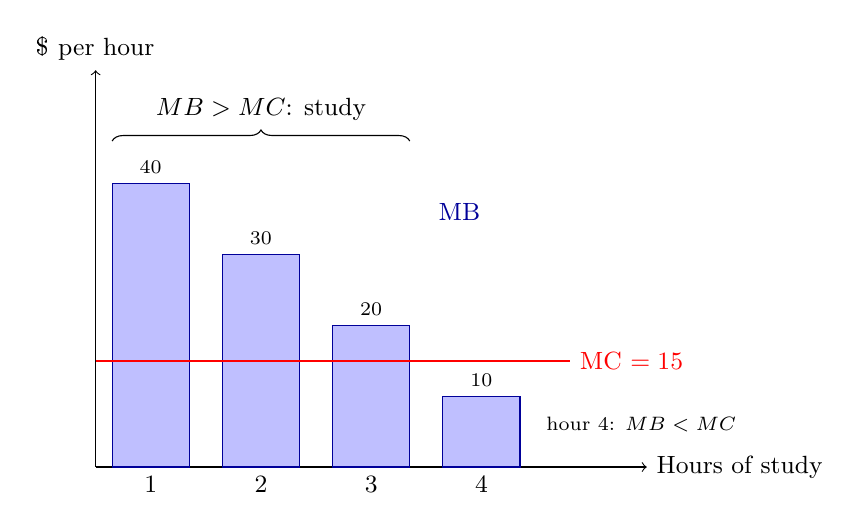
\begin{tikzpicture}[x=1.4cm, y=0.09cm, every node/.style={font=\small}]
  \draw[->] (0,0) -- (5,0) node[right] {Hours of study};
  \draw[->] (0,0) -- (0,56) node[above] {\$ per hour};
  \foreach \h/\mb in {1/40, 2/30, 3/20, 4/10} {
    \fill[blue!25] (\h-0.85,0) rectangle (\h-0.15,\mb);
    \draw[blue!60!black] (\h-0.85,0) rectangle (\h-0.15,\mb);
    \node[above, font=\scriptsize] at (\h-0.5,\mb) {\mb};
    \node[below] at (\h-0.5,0) {\h};
  }
  \draw[thick, red] (0,15) -- (4.3,15) node[right] {MC $= 15$};
  \node[blue!60!black] at (3.3,36) {MB};
  \draw[decorate, decoration={brace, amplitude=4pt}] (0.15,46) -- (2.85,46) node[midway, above=4pt] {$MB > MC$: study};
  \node[anchor=west, font=\scriptsize] at (4.0,6) {hour 4: $MB < MC$};
\end{tikzpicture}
\end{center}

\subsection{Choices respond to incentives}

A change in marginal benefit or marginal cost changes the incentives people face, and so
changes their choices. A higher tax on cigarettes raises the marginal cost of smoking and
reduces smoking. Economics predicts that people respond to incentives; it does not
assume they are selfish.

\section{Economics as a social science and policy tool}

\subsection{Positive and normative statements}

\begin{definition}[Positive vs normative]
A \emph{positive statement} is about what \emph{is}; it can be tested against the facts
(``raising the minimum wage reduces teenage employment''). A \emph{normative statement}
is about what \emph{ought to be}; it depends on values and cannot be tested (``the
minimum wage should be raised'').
\end{definition}

\subsection{Economic models}

An \emph{economic model} is a simplified description of some aspect of the economy that
includes only the features needed for the purpose at hand. Models are tested by checking
their predictions against facts. Because the economy cannot be put in a lab, economists
use natural experiments, statistical investigations and controlled lab experiments.

The key simplifying assumption is \emph{ceteris paribus} (``other things being equal''):
we change one variable at a time and hold all other influences constant.

\begin{important}[Pitfalls in economic reasoning]
\begin{itemize}
  \item \emph{Fallacy of composition}: what is true for one person is not necessarily true
        for everyone. One person standing up at a hockey game sees better; if everyone
        stands, no one does.
  \item \emph{Post hoc fallacy}: ``after this, therefore because of this.'' One event
        happening before another does not mean it caused it.
  \item Correlation is not causation.
\end{itemize}
\end{important}

\section{Graphs in economics}

Economics uses graphs with two axes to show relationships between variables.

\begin{definition}[Slope]
The \emph{slope} of a relationship is the change in the variable on the $y$-axis divided
by the change in the variable on the $x$-axis:
\[
  \text{slope} = \frac{\Delta y}{\Delta x}.
\]
A positive slope means the variables move together (\emph{positive} or \emph{direct}
relationship); a negative slope means they move in opposite directions (\emph{negative}
or \emph{inverse} relationship). A straight line has a constant slope; a curve has a
slope that varies and is measured by the tangent line at a point.
\end{definition}

\begin{example}
A line passes through $(x,y) = (2, 10)$ and $(6, 4)$. Its slope is
$\dfrac{4 - 10}{6 - 2} = \dfrac{-6}{4} = -1.5$, a negative relationship.
\end{example}

\begin{center}
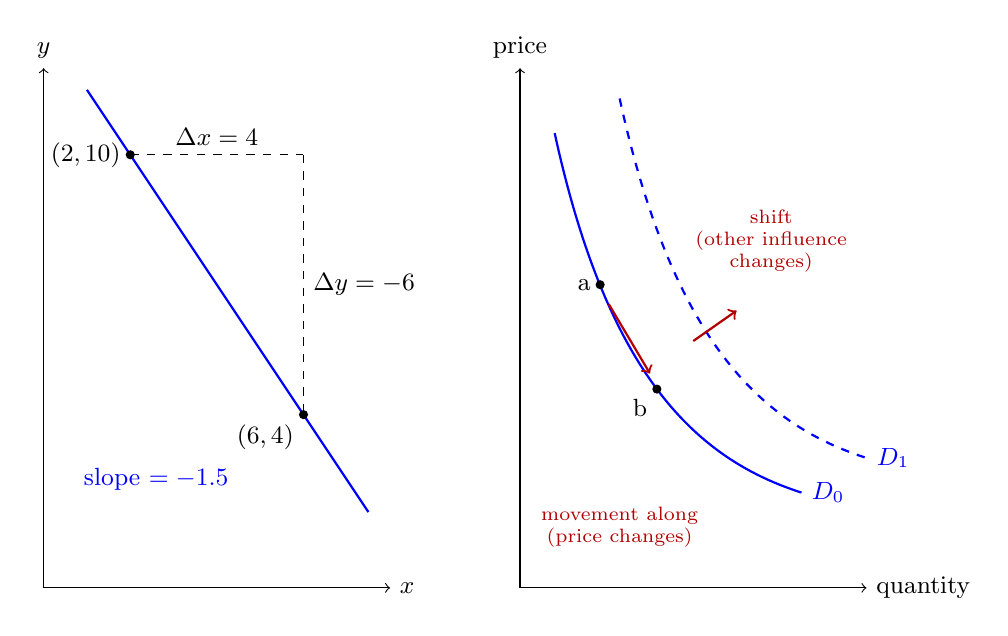
\begin{tikzpicture}[scale=0.55, every node/.style={font=\small}]
  \draw[->] (0,0) -- (8,0) node[right] {$x$};
  \draw[->] (0,0) -- (0,12) node[above] {$y$};
  \draw[thick, blue] (1,11.5) -- (7.5,1.75);
  \fill (2,10) circle (3pt) node[left] {$(2,10)$};
  \fill (6,4) circle (3pt) node[below left] {$(6,4)$};
  \draw[dashed] (2,10) -- (6,10) node[midway, above] {$\Delta x = 4$};
  \draw[dashed] (6,10) -- (6,4) node[midway, right] {$\Delta y = -6$};
  \node[blue] at (2.6,2.5) {slope $= -1.5$};
  \begin{scope}[xshift=11cm]
    \draw[->] (0,0) -- (8,0) node[right] {quantity};
    \draw[->] (0,0) -- (0,12) node[above] {price};
    \draw[thick, blue] (0.8,10.5) .. controls (2,5) and (4,3) .. (6.5,2.2) node[right] {$D_0$};
    \draw[thick, blue, dashed] (2.3,11.3) .. controls (3.5,5.8) and (5.5,3.8) .. (8,3) node[right] {$D_1$};
    \fill (1.85,7.0) circle (3pt) node[left] {a};
    \fill (3.16,4.59) circle (3pt) node[below left] {b};
    \draw[->, thick, red!70!black] (2.05,6.55) -- (3.0,4.95);
    \draw[->, thick, red!70!black] (4.0,5.7) -- (5.0,6.4);
    \node[red!70!black, align=center, font=\scriptsize] at (2.3,1.4) {movement along\\(price changes)};
    \node[red!70!black, align=center, font=\scriptsize] at (5.8,8.0) {shift\\(other influence\\changes)};
  \end{scope}
\end{tikzpicture}
\end{center}

When a variable other than the two on the axes changes, the whole curve \emph{shifts}.
This distinction (movement along a curve vs shift of the curve, right panel above) is
used throughout the course.

\section{Summary}

\begin{itemize}
  \item Scarcity forces choices; incentives influence them. Economics studies those
        choices; micro looks at individuals and markets, macro at the whole economy.
  \item Big questions: what, how and for whom are goods produced, and when does
        self-interest serve the social interest?
  \item Factors of production: land (rent), labour (wages), capital (interest),
        entrepreneurship (profit).
  \item Opportunity cost is the highest-valued alternative forgone; ignore sunk costs.
  \item Decide at the margin: do more while $MB > MC$, stop where $MB = MC$.
  \item Distinguish positive from normative statements; models rely on ceteris paribus;
        avoid the fallacy of composition and the post hoc fallacy.
\end{itemize}
